\chapter{Data Analysis}

\section{Dredging activity}
This section describes the relevance of dredging to the sediment balance of the designated area, by an estimation of the dredging volumes through different data sources. 


\subsection{Vessel positioning information (AIS)}
The number of vessels involved in dredging activities on the Paraná Guazú was determined using AIS (Automatic Identification System) data. Vessel movements between dredging sites and ports were monitored through \textit{MarineTraffic}. Although historical records were not considered, the daily activity observed during the study period provides a reliable estimate of the sand extraction volumes.

Using MarineTraffic it was found that two dredgers are operating on the Paraná Guazú between Ibicuy and Brazo Largo: the Comercio Segundo and the E.M. Arroyo N1. The Comercio Segundo has a length of 30 m, a width of 7 m, a draft of 1.3 m, and an approximate cargo hold of 195 m\textsuperscript{3}. The E.M. Arroyo N1 has a length of 39 m, a width of 8 m, a draught of 2.8 m and an approximate cargo hold of 476 \,m\textsuperscript{3}. Using a sand to water ratio of 3:1 for the dredged slurry, the amount of sand dredged is 150 \,m\textsuperscript{3} and 360 \,m\textsuperscript{3} respectively per cargo. The tracks of the two vessels obtained from MarineTraffic are shown in Figures 5.1 and 5.2.

\begin{figure}[h!]
    \centering
    \begin{minipage}{0.48\textwidth}
        \centering
        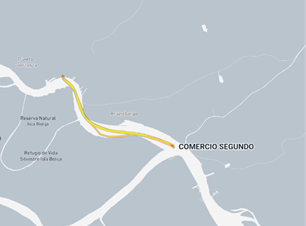
\includegraphics[width=\linewidth]{figures/figures ch5/Track_CS.png}
        \caption{Track of the \textit{Comercio Segundo}}
        \label{fig:track_cs}
    \end{minipage}\hfill
    \begin{minipage}{0.48\textwidth}
        \centering
        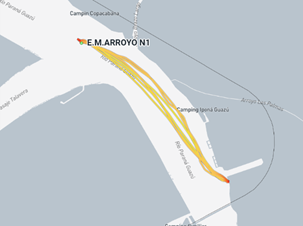
\includegraphics[width=\linewidth]{figures/figures ch5/Track_EM.png}
        \caption{Track of the \textit{E.M. Arroyo N1}}
        \label{fig:track_em}
    \end{minipage}
\end{figure}

The AIS data for these two vessels is obtained from MyShipTracking, which is used to determine the location of the dredging and the average number of trips. The dredging location of the two vessels is shown in Figure 5.3. It can be seen that both dredgers dredge in the same area. This can be explained by the bathymetry shown in Figure 5.4, which shows a reduced depth near the junction of the two navigable channels. At this location the flow velocity is lower, causing sediment to settle and thus creating a sandbar. From the AIS data it can be concluded that both dredgers make three trips per day.

\begin{figure}[h!]
    \centering
    \begin{minipage}{0.48\textwidth}
        \centering
        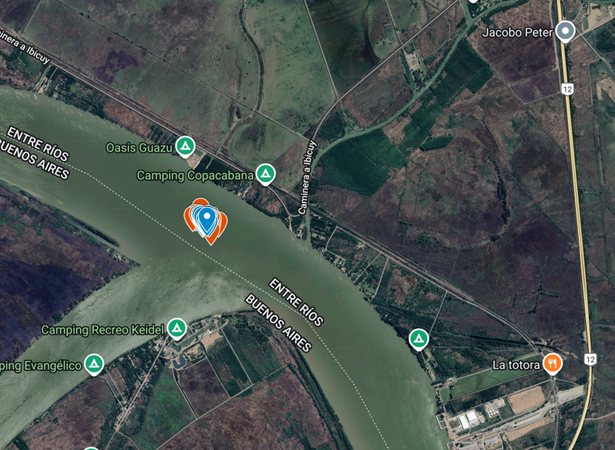
\includegraphics[width=\linewidth]{figures/figures ch5/Dredging_coordinates.png}
        \caption{Dredging location}
        \label{fig:dredging_coordinates}
    \end{minipage}\hfill
    \begin{minipage}{0.48\textwidth}
        \centering
        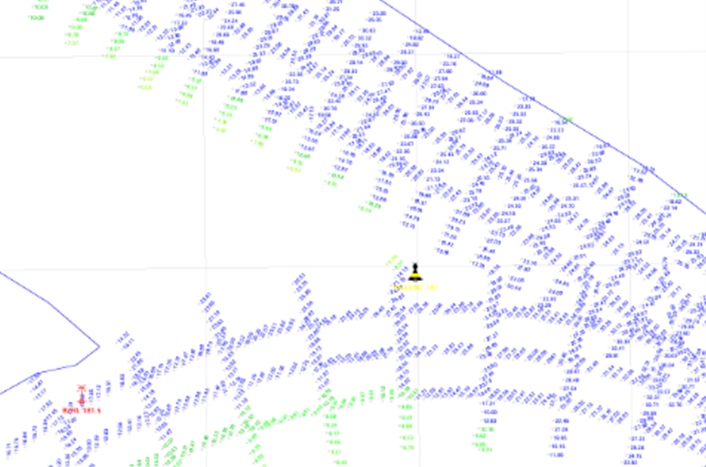
\includegraphics[width=\linewidth]{figures/figures ch5/Bathymetry.png}
        \caption{Bathymetry}
        \label{fig:bathymetry}
    \end{minipage}
\end{figure}

In the Rio Talabera, a side branch connecting to the Paraná Guazú, a third dredger is extracting sand. The Altair is dredger with a length of 66 m, a width of 11 m, a draught of 1.5 m and a approximate cargo hold of 750 \,m\textsuperscript{3}. Using the same sand to water ratio of 3:1 this gives 560 \,m\textsuperscript{3} of sand per cargo. Using MarineTraffic it was found that the Altair has an average 3 trips per day. Figure 5.5 shows the track of the Altair and the location at which it stops to extract sand. 

\begin{figure}[H]
    \centering
    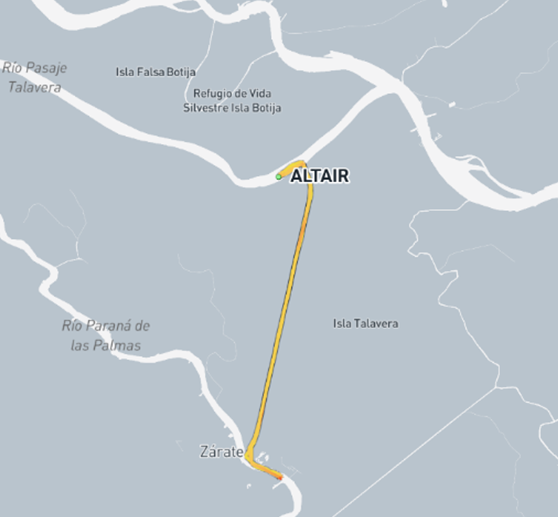
\includegraphics[width=0.5\linewidth]{figures/figures ch5/Track_Altair.png}
    \caption{Track of the Altair}
    \label{fig:placeholder}
\end{figure}

For all three vessels, the estimated volume of sand extracted per month is displayed in table 5.1
\begin{table}[h!]
\centering
\begin{tabular}{lrrrr}
\hline
\textbf{Vessel} & \textbf{Cargo hold} & \textbf{Sand volume [\,m\textsuperscript{3}]} & \textbf{Trips per day} & \textbf{Volume per month [\,m\textsuperscript{3}]} \\
\hline
Comercio Segundo & 195 & 150 & 3 & 9000 \\
E.M. Arroyo N1 & 476 & 360 & 3 & 21600 \\
Altair & 750 & 560 & 3 & 33600 \\
\hline
\end{tabular}
\caption{Sand transport details per vessel.}
\label{tab:sand_volume}
\end{table}


\subsection{Extraction permits}
To avoid adverse impacts on the hydraulic regime from dredging, companies must first obtain permits from the \textit{National Water Institute }(INA). These permits specify the locations and volumes of the proposed dredging activities. The information they provide serves as a reliable estimate of the total material being removed from the river, thereby influencing the sediment balance. Therefore, the permits were analysed for the area of interest.

A total of 33 permits were collected for the Paraná Guazú and 43 for the Ibicuy. On the Paraná Guazú, four permits were issued for channel maintenance, while the remainder concerned sand extraction. For the Ibicuy, all permits were related to extraction activities. The analysis shows that the requested volumes in the Ibicuy are considerably larger than those in the Paraná Guazú, even though the section of the Ibicuy considered here is much shorter in length.

It is important to note that the end dates of contracts are unknown. While the requests specify monthly dredging quantities, they do not indicate the duration of the works. As a result, a detailed quantitative assessment cannot be made. For the present analysis, all requests with fixed monthly volumes are assumed to extend over 12 months, allowing for a comparison between the two river sections, as shown in Figure \ref{fig:yearly dredging volumes}. The second assumption is to record a single value for the requested volume, when information about monthly or yearly occurrence is lacking.

\begin{figure}[H]
    \centering
    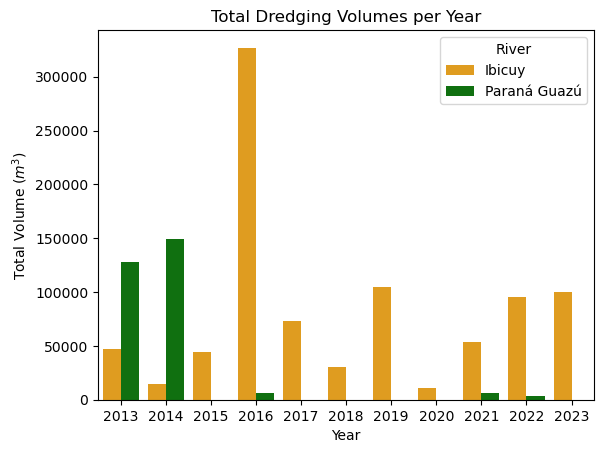
\includegraphics[width=0.50\linewidth]{figures/figure chap 2/Dredging volumes permits.png}
    \caption{Yearly dredging volumes}
    \label{fig:yearly dredging volumes}
\end{figure}

\subsection{Estimated sand extraction}

\section{Hydrodynamic data}
\section{Sediment transport}

% \section{Water Quality and Bioorganism Activity?}

